\chapter{Tecniche di Compilazione Ottimizzata e Profiling}
Come già detto più volte, per scrivere codice funzionante e ottimizzato, è importante capire bene come lavori il compilatore e come questo manipola il nostro codice per estrapolarne il meglio.

\section{Compilatore}
Il \textbf{compilatore} è un programma che traduce il linguaggio sorgente in un linguaggio target equivalente.
Questo è importante per il calcolo HPC perché funge da intermediario tra codice e hardware. Inoltre, un buon compilatore riesce a ottimizzare altamente il codice che abbiamo scritto per una specifica architetture proprio per garantire delle ottime prestazioni. 
Comprenderne i limiti, infatti, ci permetterà di scrivere codice che può essere ottimizzato ancora meglio dal compilatore stesso.

Un \textbf{interprete}, al contrario di quanto fa un compilatore, è un programma di elaborazione del linguaggio che esegue \textbf{direttamente} un programma in un \textbf{linguaggio sorgente}.

Questo risulta generalmente in un codice più portabile ma che, nel caso del calcolo HPC non torna molto utile poiché l'ottimizzazione su macchine specifiche è un grosso vantaggio in termini di prestazioni generali del programma.

\subsection{Pipeline di Compilazione}
La compilazione fa parte di una \textbf{pipeline} che traduce il codice sorgente in un codice eseguibile dalla macchina. 
Questa pipeline comprende:
\begin{itemize}
    \item \textbf{Preprocessore}: Analizza il sorgente includendo gli header ed espandendo le macro. Gli Header non sono altro che dei file al cui interno contengono solo la dichiarazione della funzione ma non il suo corpo.
    \item \textbf{Front-end o Compilazione (in base alla slide che stai leggendo)}: Traduce il sorgente in un linguaggio ad alto livello di astrazione, assembly nello specifico. Qui vengono anche effettuate le prime analisi sintattiche e semantiche del programma.
    \item \textbf{Assembler}: Produce il codice macchina dall'assemby generato alla fase precedente risolvendo label interni e lasciando quelli esterni ancora irrisolti.
    \item \textbf{Linker}: Risolve i riferimenti e gli indirizzi di memoria tra diverse sezioni del codice e librerie esterne.
\end{itemize}
\begin{figure}[H]
    \centering
    
\includegraphics[width=0.7\linewidth]{Images/cap_7/pipeline_compilazione.png}
\end{figure}
I moderni compilatori sono anche in grado di applicare trasformazioni al codice per migliorarne le prestazioni:
\begin{itemize}
    \item \textbf{Constant folding}: calcola espressioni costanti a tempo di compilazione.
    \item \textbf{Dead code elimination}: rimuove codice irraggiungibile o mai utilizzato.
    \item \textbf{Inlining delle funzioni}: sostituisce le chiamate con il corpo della funzione.
    \item \textbf{Loop unrolling}: replica il corpo del ciclo per ridurre il controllo del loop.
    \item \textbf{Common subexpression elimination}: evita di ricalcolare la stessa espressione.
    \item \textbf{Vettorizzazione automatica}: usa istruzioni SIMD (SSE, AVX) su array.
    \item \textbf{Instruction scheduling}: riordina le istruzioni per sfruttare la pipeline della CPU.
    \item \textbf{Register allocation}: minimizza gli accessi in memoria usando i registri della CPU.
\end{itemize}

I compilatori moderni (come GCC o Clang) offrono diversi "preset" di ottimizzazione che bilanciano velocità di compilazione, facilità di debug e performance del codice eseguibile.

\begin{itemize}
    \item \textbf{-O0 (Nessuna ottimizzazione)}:
        \begin{itemize}
        \item Offre una compilazione molto veloce e un debug semplificato, poiché ogni istruzione C corrisponde a poche istruzioni assembly.
        \item Il codice risultante è più lento ma completamente prevedibile, rendendolo ideale per l'uso durante lo sviluppo con strumenti come \textit{gdb}.
    \end{itemize}

    \item \textbf{-O1 (Ottimizzazioni di base)}:
    \begin{itemize}
        \item Riduce le dimensioni dell'eseguibile e i tempi di esecuzione senza allungare significativamente i tempi di compilazione.
        \item Include l'eliminazione di variabili inutili e l'ottimizzazione dei salti.
        \item Per loop semplici, può risultare già 2 o 5 volte più veloce rispetto a -O0.
    \end{itemize}

    \item \textbf{-O2 (Ottimizzazioni raccomandate)}:
    \begin{itemize}
        \item Rappresenta lo standard per i rilasci ufficiale e il punto di partenza corretto per il codice in produzione.
        \item Attiva quasi tutte le ottimizzazioni considerate "sicure", come la vettorizzazione, la \textit{Common Subexpression Elimination} (CSE) e le trasformazioni dei loop.
    \end{itemize}

    \item \textbf{-O3 (Ottimizzazioni aggressive)}:
    \begin{itemize}
        \item Introduce l'inlining aggressivo e altre tecniche che possono aumentare la dimensione del codice (\textit{code bloat}).
        \item È necessario testare attentamente le prestazioni poiché su codici di grandi dimensioni può risultare più lento di -O2 a causa di effetti negativi sulla cache.
    \end{itemize}

    \item \textbf{-Ofast (Aggressivo + FP non-standard)}:
    \begin{itemize}
        \item Include tutte le ottimizzazioni di -O3 più il flag \textit{-ffast-math}.
        \item Permette il riordinamento delle operazioni in virgola mobile violando lo standard IEEE 754.
        \item \textbf{Attenzione}: Può alterare i risultati numerici; non deve mai essere usato in codice scientifico senza una validazione accurata dei risultati.
    \end{itemize}
    \item \textbf{-Os (Ottimizzazione per dimensioni)}: Sebbene nel calcolo HPC questa non risulti particolarmente utile, è giusto segnalarla. Si tratta di ottimizzazioni che non cercano di aumentare le prestazioni del sistema in termini di tempo ma in termini di dimensione del codice. Spesso utilizzato per i microcontrollori.
    \item \textbf{-march=native}: Istruisce il compilatore a generare codice specifico per l'architettura della CPU su cui sta girando, sfruttando tutti i set di istruzioni (ISA) disponibili. Infatti, il compilatore generalmente produce un codice portabile, cioè un codice che può essere eseguito su qualsiasi CPU appartenente a quella classe di architettura.
\end{itemize}

\subsection{Il Memory Aliasing}
Il \textbf{Memory Aliasing} si verifica quando due o più riferimenti (puntatori) puntano alla stessa posizione di memoria. Questo è uno dei maggiori blocchi alle prestazioni in C/C++.
\begin{figure}[H]
    \centering
    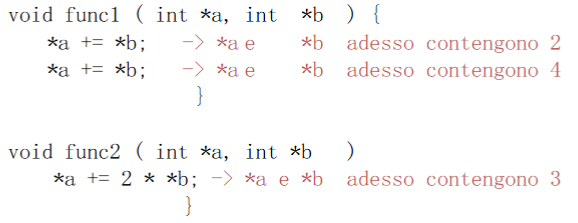
\includegraphics[width=0.75\linewidth]{Images/cap_3/aliasing.png}
\end{figure}
Consideriamo queste due funzioni. In effetti, se a e b puntano a due indirizzi diversi, il risultato delle due funzioni è lo stesso. Il discorso cambia, invece, quando a e b puntano allo stesso indirizzo come mostrato in figura.

Allo stesso modo accade nel seguente codice:
\begin{verbatim}
    void scale(double *a,double *b, int n, double s){
        for(int i = 0; i<n;i++) 
        a[i] = s * b[i-1];
    }
\end{verbatim}

Se il compilatore non può garantire che due puntatori siano distinti, non può ottimizzare gli accessi alla memoria perché teme che una scrittura su uno possa influenzare il valore dell'altro. 

Questo costringe la CPU a ricaricare continuamente i dati dalla memoria centrale anziché usare i registri o la cache. Per risolvere questo problema usiamo il qualificatore \textit{restrict}.
Esistono anche due flag:
\begin{itemize}
    \item \texttt{-fstrict-aliasing}: questo flag dice al compilatore che non possono esserci aliasing tra tipi diversi. È di default nel caso di $-O2$
    \item \texttt{-fno-strict-aliasing}: serve a dire al compilatore di non assumere che non ci siano sovrapposizioni in nessun caso.
\end{itemize}

Esistono molti altri quantificatori che aiutano il compilatore:
\begin{itemize}
    \item \textbf{Const}: Questo dice al nostro compilatore che il valore di questa variabile non cambierà nello scope corrente permettendogli, dunque, di tenere il valore in registro senza leggerlo più volte dalla memoria. 
    \item \textbf{restrict}: Ne abbiamo già parlato prima, dice al compilatore che quel puntatore punta a un indirizzo di memoria esclusivamente puntato da lui.
    \item \textbf{volatile}: informa il compilatore che quel valore potrebbe cambiare inaspettatamente, così facendo, il compilatore ne impedisce il caching in registro e riordinamento delle istruzioni.
    \item \textbf{register}: suggerisce al compilatore che quella variabile verrà usata spesso e quindi deve tenerla in registro. Suggerimento che potrebbe essere tranquillamente ignorato dal compilatore poiché in genere se ne occupa lui in maniera più efficiente.
\end{itemize}
Esistono anche diverse classi di storage:
\begin{itemize}
    \item \textbf{extern}: variabili globali che esistono per tutta la durata del programma.
    \item \textbf{auto}: variabili locali allocate sullo stack e distrutte subito dopo l'uscita dal blocco.
    \item \textbf{static}: variabili che persistono tra le varie chiamate a funzioni. Sono visibili solo all'interno del file corrente e permettono di evitare reinizializzazioni e abilita il caching.
\end{itemize}
In generale, nel caso in cui volessimo analizzare l'assembly del nostro codice, esistono diversi strumenti tra cui \textbf{godbolt, perf annote} o, banalmente, \textbf{gcc -S -fverobse-asm}.

\section{Profiling}
Il profiling rappresenta il cuore del Performance Engineering. Consiste nell'analizzare l'esecuzione di un programma utilizzando carichi di lavoro (workload) reali per identificare con precisione gli hotspots (punti critici) e i bottleneck (colli di bottiglia) del codice.

Senza una misurazione oggettiva, l'ottimizzazione rischierebbe di basarsi su intuizioni spesso errate; profilare ci permette invece di quantificare i problemi per intervenire dove è realmente necessario.

Il ciclo iterativo del Performance Engineering si articola in quattro fasi:
\begin{itemize}
    \item \textbf{Profilare}: Individuare i colli di bottiglia basandosi su dati di esecuzione reali.
    \item \textbf{Analizzare}: Studiare il codice per comprendere la causa radice del rallentamento (es. problemi di cache, algoritmi inefficienti, contesa di memoria).
    \item \textbf{Ottimizzare}: Implementare le modifiche mirate per risolvere il problema identificato.
    \item \textbf{Verificare}: Misurare nuovamente le prestazioni per convalidare il miglioramento ed escludere eventuali regressioni.
\end{itemize}

È fondamentale non procedere all'ottimizzazione basandosi sull'intuito, bensì su misurazioni concrete. Spesso sappiamo che il $90\%$ del tempo di esecuzione è concentrato nel $10\%$ del codice: è proprio da quegli hotspot che dobbiamo partire per massimizzare l'impatto del nostro lavoro.Idealmente, un processo di profiling efficace deve fornire risposte a domande precise:
\begin{itemize}
    \item \textbf{Hotspots}: Quali sezioni di codice consumano la maggior parte del tempo totale?
    \item \textbf{Cache Efficiency}: Quanti \textit{cache miss} si verificano e in quali loop la memoria diventa il collo di bottiglia?
    \item \textbf{Pipeline Utilization}: La CPU sta sfruttando correttamente la \textit{pipeline} o si verificano stalli frequenti?
    \item \textbf{Throughput}: Quante istruzioni vengono effettivamente ritirate per ciclo di clock (IPC)?
    \item \textbf{Performance Bound}: Il codice è \textbf{compute bound} (limitato dalla capacità di calcolo) o \textbf{memory bound} (limitato dalla velocità della memoria)?
\end{itemize}
\subsection{PMU}
I moderni processori contengono hardware dedicato al monitoraggio delle proprie prestazioni. Sono circuiti integrati nella CPU che contano eventi micro architetturali con precisione.
Questi sono parecchio utili:
\begin{itemize}
    \item \textbf{Efficienza}: Garantisce un \textbf{overhead minimo} ($< 1\%$), permettendo misurazioni in tempo reale senza degradare significativamente le prestazioni del sistema.
    \item \textbf{Precisione Fisica}: Crea una correlazione diretta tra l'esecuzione del software e le caratteristiche fisiche della CPU, individuando le cause profonde dei colli di bottiglia.
    \item \textbf{Portabilità}: Grazie all'astrazione fornita dai tool moderni, è possibile raccogliere metriche hardware senza dover gestire manualmente i registri specifici di ogni diversa microarchitettura.
\end{itemize}

La PMU opera coordinando due tipologie principali di registri hardware, che lavorano in coppia per ogni "canale" di monitoraggio attivo:

\begin{itemize}
    \item \textbf{Performance Event Select Register (PESR)}: Rappresenta il "pannello di controllo" dell'evento.
    \begin{itemize}
        \item \textbf{Configurazione}: Definisce \textit{quale} evento monitorare (Event Select) e con quale specifica variante (Unit Mask).
        \item \textbf{Filtraggio}: Contiene i bit di controllo per stabilire se il conteggio deve avvenire solo in modalità Utente, solo in Kernel, o in entrambe.
        \item \textbf{Attivazione}: Funge da interruttore per far partire o fermare il monitoraggio del relativo contatore.
    \end{itemize}

    \item \textbf{Performance Monitor Counter (PMC)}: È il contatore digitale vero e proprio associato al PESR.
    \begin{itemize}
        \item \textbf{Accumulazione}: Incrementa il proprio valore ogni volta che l'evento configurato nel PESR si verifica a livello microarchitetturale.
        \item \textbf{Sampling (Interrupt su Overflow)}: Questa è la sua funzione più potente. Quando il registro raggiunge il suo valore massimo (overflow), può generare un interrupt hardware. Questo permette al sistema operativo di "fotografare" esattamente quale istruzione stava girando in quel momento, permettendo il profiling statistico (campionamento).
    \end{itemize}
\end{itemize}

I tipi di eventi monitorabili sono:
\begin{itemize}
    \item \textbf{Istruzioni ritirate (INST\_RETIRED)}: Indica il numero di istruzioni completate con successo dal processore. È una metrica fondamentale per misurare il lavoro utile effettivamente svolto.
    \item \textbf{Cicli di clock (CPU\_CLK\_UNHALTED)}: Rappresenta i cicli totali in cui la CPU è in stato attivo e non in stop. Combinato con le istruzioni ritirate, permette di calcolare l'IPC (\textit{Instructions Per Cycle}).
    \item \textbf{Cache miss (LLC\_MISSES, L1D\_MISSES)}: Conteggia gli accessi falliti ai vari livelli di cache, come la L1 o la LLC (\textit{Last Level Cache}). Alti valori qui indicano solitamente un codice \textit{memory bound}.
    \item \textbf{Branch misprediction (BR\_MISP\_RETIRED)}: Misura gli errori di predizione del \textit{branch predictor} hardware. Ogni errore causa lo svuotamento della pipeline, con una pesante penalità in termini di cicli persi.
    \item \textbf{TLB miss (D-TLB, I-TLB MISSES)}: Registra i fallimenti nella traduzione hardware degli indirizzi virtuali. Un numero elevato di questi eventi suggerisce che il programma sta accedendo alla memoria in modo troppo sparso su molte pagine diverse.
    \item \textbf{Stalli della pipeline (RESOURCE\_STALLS)}: Indica i cicli persi a causa di dipendenze di dati tra istruzioni o conflitti strutturali all'interno della CPU.
\end{itemize}

I contatori possono essere usati in due modalità:
\begin{itemize}
    \item \textbf{Counting mode:} Contiamo il numero esatto di eventi in un intervallo di codice. Avremo overhead minimo, risultati precisi, ideale per misure globali.
    \item \textbf{Sampling mode:} Il PMC genera un interrupt ogni N eventi, registrando l'istruzione corrente. Permette di identificare gli hotspot nel codice.
\end{itemize}

\subsubsection{Performance Events for Linux (Perf)}
Perf è l'infrastruttura standard di profiling su Linux, integrata nel kernel (v2.6+). Astrae le differenze hardware tra CPU offrendo un'interfaccia a riga di comando unificata.
Perf è composto da due componenti:
\begin{itemize}
    \item \textbf{Kernel SYSCALL}: Questo, attraverso la chiamata \texttt{perf\_event\_open()} permette un accesso unificato agli eventi del SO e agli eventi hardware PMU del processore.
    \item \textbf{User-space tools}: Questi sono i comandi utilizzabili da CLI per raccogliere e analizzare i dati. 
\end{itemize}
perf permette di spiare dettagli “intimi” del sistema e quindi richiede privilegi. È necessario abbassare temporaneamente le restrizioni del kernel:
\begin{figure}[H]
    \centering
    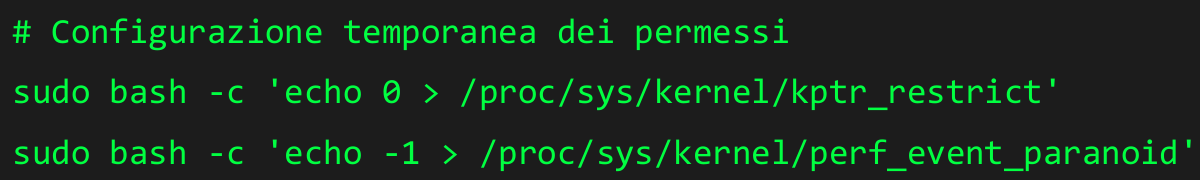
\includegraphics[width=0.5\linewidth]{Images/cap_7/comandi.png} 
\end{figure}
Esistono vari tipi di eventi che possiamo monitorare tramite perf:
\begin{itemize}
    \item \textbf{Software events}: Si tratta di eventi generati interamente dal kernel del sistema operativo tramite software. Includono operazioni come:
    \begin{itemize}
        \item \textit{context-switches}: i cambi di contesto tra processi.
        \item \textit{cpu-migrations}: lo spostamento di un task da una CPU a un'altra.
        \item \textit{page-faults}: errori di pagina nella gestione della memoria.
        \item \textit{task-clock}: il tempo di CPU effettivamente consumato dal task.
    \end{itemize}

    \item \textbf{Hardware events (PMU)}: Sono eventi mappati su reali contatori hardware presenti nel processore. Hanno il vantaggio di essere portatili tra diverse architetture e comprendono:
    \begin{itemize}
        \item \textit{cycles}: cicli di clock della CPU.
        \item \textit{instructions}: numero di istruzioni eseguite.
        \item \textit{cache-references / cache-misses}: accessi e fallimenti nei vari livelli di cache.
        \item \textit{branch-misses}: errori di predizione dei salti.
    \end{itemize}

    \item \textbf{Hardware cache events}: Forniscono un accesso strutturato e specifico agli eventi legati alle gerarchie di cache. Esempi tipici sono:
    \begin{itemize}
        \item \textit{L1-dcache-loads / L1-dcache-load-misses}: letture e fallimenti nella cache dati di primo livello.
        \item \textit{LLC-loads / LLC-load-misses}: accessi alla \textit{Last Level Cache} (solitamente L3).
    \end{itemize}

    \item \textbf{Tracepoint events}: Sono eventi implementati tramite l'infrastruttura \texttt{ftrace} del kernel. Permettono di tracciare in modo dettagliato chiamate di sistema (\textit{syscall}), operazioni di input/output (I/O) ed eventi legati allo \textit{scheduler}.
\end{itemize}

Per identificare gli eventi disponibili sul sistema, si utilizza il comando \texttt{perf list}, che può essere filtrato tramite \texttt{grep} per isolare categorie specifiche (es. \texttt{perf list | grep cache}).

\subsubsection*{1. Counting Mode: \texttt{perf stat}}
Il comando \texttt{perf stat} esegue il programma in modalità \textit{counting}, fornendo un riepilogo aggregato degli eventi al termine dell'esecuzione.

\begin{itemize}
    \item \textbf{Utilizzo}: \texttt{perf stat ./programma}.
    \item \textbf{Metriche Chiave}: Una delle più importanti è l'IPC (Instructions Per Cycle).
    \begin{itemize}
        \item \textbf{IPC tra 1 e 4}: Indica un buon utilizzo della pipeline (architettura superscalare).
        \item \textbf{IPC < 1}: Segnala la presenza di stalli frequenti (es. attesa della memoria o errori di predizione).
    \end{itemize}
    \item \textbf{Opzioni utili}:
    \begin{itemize}
        \item \texttt{-e <event>}: Filtra la visualizzazione per mostrare solo eventi specifici.
        \item \texttt{-r <n>}: Ripete la misura $n$ volte per calcolare una media robusta.
        \item \texttt{-p <pid>}: Analizza un processo già in esecuzione.
        \item \texttt{-a -C <core\_id>}: Monitora l'attività su core specifici.
    \end{itemize}
\end{itemize}

\subsubsection*{2. Sampling Mode: \texttt{perf record} e \texttt{report}}
A differenza del counting, la modalità \textit{sampling} tramite \texttt{perf record} genera un campione statistico che permette di localizzare esattamente gli hotspot nel codice.

\begin{itemize}
    \item \textbf{Simboli di Debug}: È fondamentale compilare il codice con il flag \texttt{-g} per includere i simboli di debug; senza di essi, \texttt{perf} non potrebbe correlare i campioni alle righe del codice sorgente C.
    \item \textbf{Workflow}:
    \begin{enumerate}
        \item \texttt{perf record ./programma}: Registra i campioni in un file (\texttt{perf.data}).
        \item \texttt{perf report}: Visualizza un istogramma delle funzioni in cui il processo spende più tempo.
        \item \texttt{perf annotate}: Permette di scendere nel dettaglio e vedere i campioni riga per riga (sia sorgente C che assembly).
        \item \texttt{perf diff}: Consente di confrontare due diverse esecuzioni (es. prima e dopo un'ottimizzazione) per verificarne l'efficacia.
    \end{enumerate}
\end{itemize}

\subsubsection*{3. Call Graph Analysis}
Mentre il "flat profiling" mostra solo quali funzioni sono lente, la Call Graph Analysis permette di risalire alla gerarchia delle chiamate per capire \textit{chi} ha invocato la funzione critica.

\begin{itemize}
    \item \textbf{Comando}: \texttt{perf record -g --call-graph dwarf ./prog} (l'opzione \textit{dwarf} usa i simboli di debug per ricostruire lo stack).
    \item \textbf{Visualizzazione}: \texttt{perf report --call-graph --stdio}.
    \item \textbf{Utilità}: Identifica le cosiddette \textbf{funzioni "trampolino"} (o wrapper), ovvero funzioni che presentano un alto overhead \textit{totale} (somma delle funzioni chiamate) ma un basso overhead \textit{proprio} (lavoro svolto direttamente). Questo è essenziale per capire se il problema è la funzione stessa o il modo in cui viene invocata ripetutamente.
\end{itemize}

\subsubsection{Altri strumenti di Profiling}
Sebbene \texttt{perf} sia uno strumento eccellente per l'analisi a livello di sistema, esistono alternative che offrono vantaggi specifici come l'integrazione programmatica, la facilità d'uso per l'heap profiling o analisi specializzate per il calcolo parallelo. 

\subsubsection*{PAPI (Performance Application Programming Interface)}
PAPI è una libreria open source che offre un'interfaccia portabile per accedere agli hardware performance counter direttamente dall'interno del codice applicativo.

\begin{itemize}
    \item \textbf{Vantaggi rispetto a \texttt{perf}}: Consente un "profiling chirurgico" (misurando solo specifiche sezioni di codice), garantisce portabilità su diverse architetture (x86, ARM, IBM POWER) ed è ideale per creare benchmark ripetibili.
    \item \textbf{Integrazione e Utilizzo}: Richiede l'inizializzazione degli eventi, seguita dall'inserimento delle funzioni \texttt{PAPI\_start()} e \texttt{PAPI\_stop()} attorno alla porzione di codice da analizzare. Per la compilazione, è necessario linkare la libreria aggiungendo il flag \texttt{-lpapi}.
\end{itemize}

\subsubsection*{gperftools (Google Performance Tools)}
È una suite sviluppata da Google, considerata più semplice di \texttt{perf}, che include un profiler per la CPU (basato sul campionamento) e un heap profiler.

\begin{itemize}
    \item \textbf{Modalità d'uso}:
    \begin{itemize}
        \item \textit{Senza modifiche al codice (Preload)}: Utilizzando la variabile d'ambiente \texttt{LD\_PRELOAD=/path/libprofiler.so} seguita dall'esecuzione del programma.
        \item \textit{Con integrazione nel codice}: Includendo la libreria (\texttt{\#include <gperftools/profiler.h>}), avvolgendo il codice tra \texttt{ProfilerStart()} e \texttt{ProfilerStop()}, e compilando con il flag \texttt{-lprofiler}.
    \end{itemize}
    \item \textbf{Analisi dei dati}: Si effettua tramite il tool \texttt{pprof}, che permette di generare output testuali, dettagli riga per riga, o visualizzazioni grafiche consultabili direttamente nel browser.
\end{itemize}

\subsubsection*{Confronto e Regola Pratica di Profiling}
La scelta dello strumento dipende dal livello di dettaglio e dall'obiettivo dell'analisi:

\begin{itemize}
    \item \textbf{\texttt{perf stat}}: Non richiede modifiche al codice e fornisce una misura globale degli eventi hardware, ideale per comprendere il comportamento complessivo (es. IPC, cache miss rate).
    \item \textbf{\texttt{perf record} + \texttt{perf report}}: Profiling per campionamento utile per identificare le catene di chiamate (call chains) e scoprire esattamente in quali funzioni l'applicazione spende più tempo (hotspot).
    \item \textbf{PAPI}: Ottimo per benchmark scientifici e misurazioni precise, sebbene richieda la modifica del codice sorgente.
    \item \textbf{gperftools}: Ottimo compromesso tra semplicità di integrazione e livello di dettaglio per identificare rapidamente i colli di bottiglia in applicazioni complesse.
\end{itemize}

\textbf{Workflow Consigliato} \\
Per un'analisi efficace delle prestazioni, la regola pratica suggerisce di procedere per gradi:
\begin{enumerate}
    \item Iniziare sempre con \textbf{\texttt{perf stat}} per avere una visione d'insieme delle performance.
    \item Utilizzare \textbf{\texttt{perf record}} per localizzare e isolare gli hotspot.
    \item Impiegare \textbf{PAPI o gperftools} per effettuare misurazioni chirurgiche e dettagliate solo all'interno delle sezioni critiche individuate.
\end{enumerate}